% SOURCE: edit-harness/results/frame_a/cells/cell_*_real_MIX_C_*.json
% !TEX encoding = UTF-8 Unicode
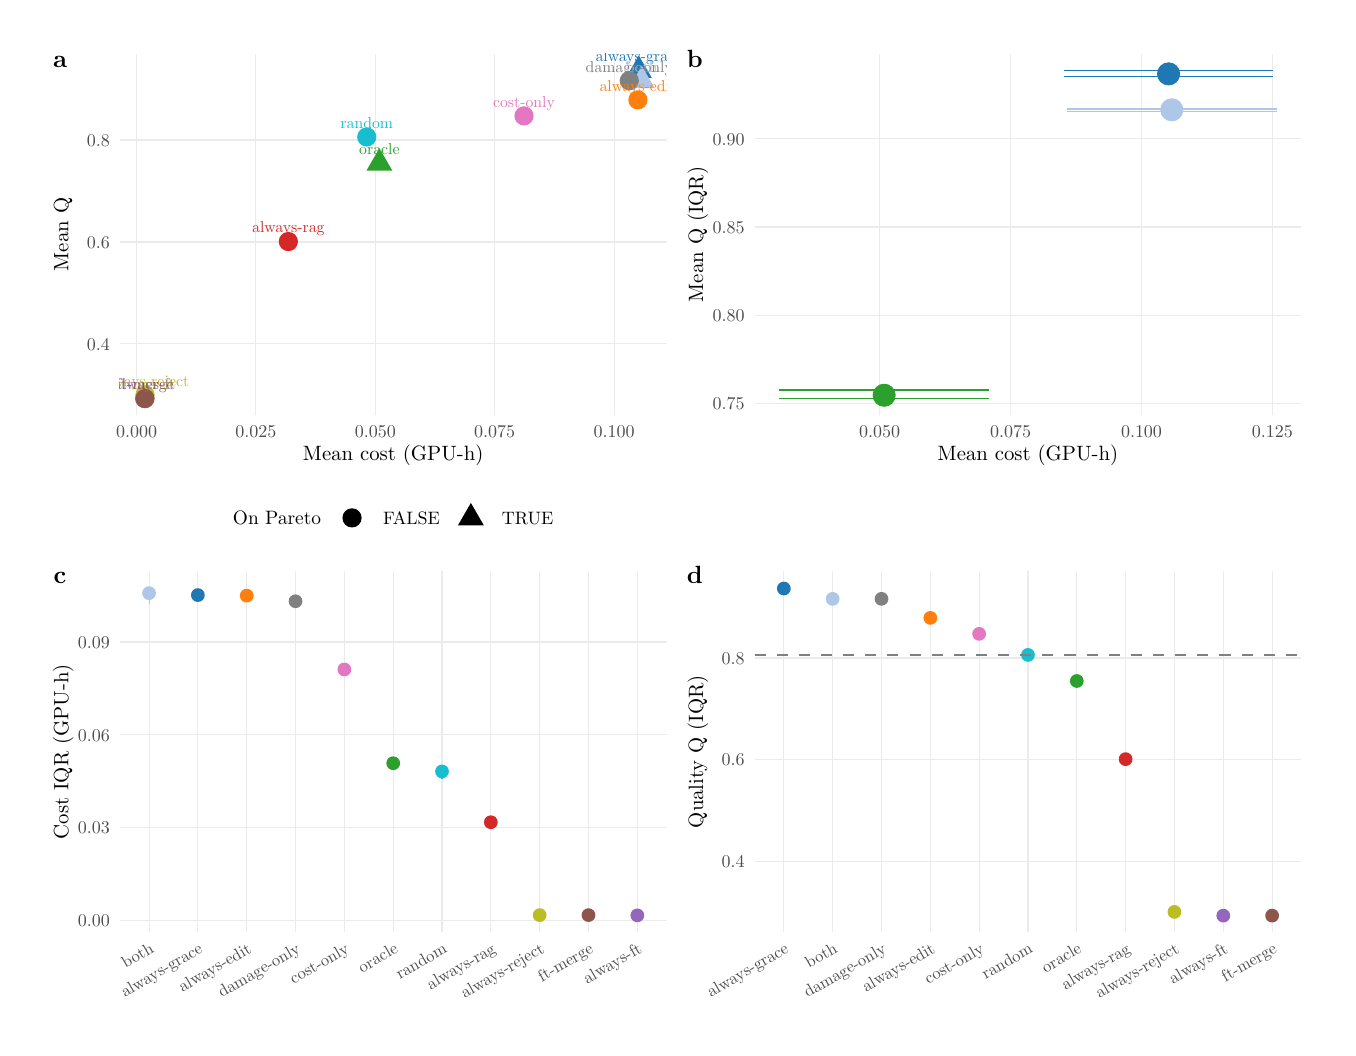
\begin{tikzpicture}[x=1pt,y=1pt]
\definecolor{fillColor}{RGB}{255,255,255}
\path[use as bounding box,fill=fillColor,fill opacity=0.00] (0,0) rectangle (469.75,361.35);
\begin{scope}
\path[clip] (  0.00,  0.00) rectangle (469.75,361.35);
\definecolor{drawColor}{RGB}{255,255,255}
\definecolor{fillColor}{RGB}{255,255,255}

\path[draw=drawColor,line width= 0.6pt,line join=round,line cap=round,fill=fillColor] (  0.00,  0.00) rectangle (469.75,361.35);
\end{scope}
\begin{scope}
\path[clip] (  5.50,168.99) rectangle (234.88,355.85);
\definecolor{fillColor}{RGB}{255,255,255}

\path[fill=fillColor] (  5.50,168.99) rectangle (234.88,355.85);
\end{scope}
\begin{scope}
\path[clip] (234.88,168.99) rectangle (464.25,355.85);
\definecolor{fillColor}{RGB}{255,255,255}

\path[fill=fillColor] (234.88,168.99) rectangle (464.25,355.85);
\end{scope}
\begin{scope}
\path[clip] (  5.50,  5.50) rectangle (234.88,168.99);
\definecolor{fillColor}{RGB}{255,255,255}

\path[fill=fillColor] (  5.50,  5.50) rectangle (234.88,168.99);
\end{scope}
\begin{scope}
\path[clip] (234.88,  5.50) rectangle (464.25,168.99);
\definecolor{fillColor}{RGB}{255,255,255}

\path[fill=fillColor] (234.88,  5.50) rectangle (464.25,168.99);
\end{scope}
\begin{scope}
\path[clip] ( 33.28,221.41) rectangle (230.88,351.85);
\definecolor{drawColor}{gray}{0.92}

\path[draw=drawColor,line width= 0.4pt,line join=round] ( 33.28,247.09) --
	(230.88,247.09);

\path[draw=drawColor,line width= 0.4pt,line join=round] ( 33.28,283.91) --
	(230.88,283.91);

\path[draw=drawColor,line width= 0.4pt,line join=round] ( 33.28,320.74) --
	(230.88,320.74);

\path[draw=drawColor,line width= 0.4pt,line join=round] ( 39.33,221.41) --
	( 39.33,351.85);

\path[draw=drawColor,line width= 0.4pt,line join=round] ( 82.47,221.41) --
	( 82.47,351.85);

\path[draw=drawColor,line width= 0.4pt,line join=round] (125.62,221.41) --
	(125.62,351.85);

\path[draw=drawColor,line width= 0.4pt,line join=round] (168.76,221.41) --
	(168.76,351.85);

\path[draw=drawColor,line width= 0.4pt,line join=round] (211.91,221.41) --
	(211.91,351.85);
\definecolor{fillColor}{RGB}{255,127,14}

\path[fill=fillColor] (220.50,335.26) circle (  3.47);
\definecolor{fillColor}{RGB}{148,103,189}

\path[fill=fillColor] ( 42.26,227.33) circle (  3.47);
\definecolor{fillColor}{RGB}{31,119,180}

\path[fill=fillColor] (220.83,351.32) --
	(225.51,343.22) --
	(216.15,343.22) --
	cycle;
\definecolor{fillColor}{RGB}{214,39,40}

\path[fill=fillColor] ( 94.20,284.06) circle (  3.47);
\definecolor{fillColor}{RGB}{188,189,34}

\path[fill=fillColor] ( 42.40,228.68) circle (  3.47);
\definecolor{fillColor}{RGB}{174,199,232}

\path[fill=fillColor] (221.90,347.57) --
	(226.57,339.47) --
	(217.22,339.47) --
	cycle;
\definecolor{fillColor}{RGB}{227,119,194}

\path[fill=fillColor] (179.35,329.48) circle (  3.47);
\definecolor{fillColor}{gray}{0.50}

\path[fill=fillColor] (217.39,342.17) circle (  3.47);
\definecolor{fillColor}{RGB}{140,86,75}

\path[fill=fillColor] ( 42.40,227.33) circle (  3.47);
\definecolor{fillColor}{RGB}{44,160,44}

\path[fill=fillColor] (127.09,317.79) --
	(131.77,309.69) --
	(122.42,309.69) --
	cycle;
\definecolor{fillColor}{RGB}{23,190,207}

\path[fill=fillColor] (122.53,321.85) circle (  3.47);
\definecolor{drawColor}{RGB}{255,127,14}

\node[text=drawColor,anchor=base,inner sep=0pt, outer sep=0pt, scale=  0.57] at (220.50,338.40) {always-edit};
\definecolor{drawColor}{RGB}{148,103,189}

\node[text=drawColor,anchor=base,inner sep=0pt, outer sep=0pt, scale=  0.57] at ( 42.26,230.47) {always-ft};
\definecolor{drawColor}{RGB}{31,119,180}

\node[text=drawColor,anchor=base,inner sep=0pt, outer sep=0pt, scale=  0.57] at (220.83,349.06) {always-grace};
\definecolor{drawColor}{RGB}{214,39,40}

\node[text=drawColor,anchor=base,inner sep=0pt, outer sep=0pt, scale=  0.57] at ( 94.20,287.20) {always-rag};
\definecolor{drawColor}{RGB}{188,189,34}

\node[text=drawColor,anchor=base,inner sep=0pt, outer sep=0pt, scale=  0.57] at ( 42.40,231.82) {always-reject};
\definecolor{drawColor}{RGB}{174,199,232}

\node[text=drawColor,anchor=base,inner sep=0pt, outer sep=0pt, scale=  0.57] at (221.90,345.31) {both};
\definecolor{drawColor}{RGB}{227,119,194}

\node[text=drawColor,anchor=base,inner sep=0pt, outer sep=0pt, scale=  0.57] at (179.35,332.62) {cost-only};
\definecolor{drawColor}{gray}{0.50}

\node[text=drawColor,anchor=base,inner sep=0pt, outer sep=0pt, scale=  0.57] at (217.39,345.31) {damage-only};
\definecolor{drawColor}{RGB}{140,86,75}

\node[text=drawColor,anchor=base,inner sep=0pt, outer sep=0pt, scale=  0.57] at ( 42.40,230.47) {ft-merge};
\definecolor{drawColor}{RGB}{44,160,44}

\node[text=drawColor,anchor=base,inner sep=0pt, outer sep=0pt, scale=  0.57] at (127.09,315.53) {oracle};
\definecolor{drawColor}{RGB}{23,190,207}

\node[text=drawColor,anchor=base,inner sep=0pt, outer sep=0pt, scale=  0.57] at (122.53,324.98) {random};
\end{scope}
\begin{scope}
\path[clip] (  0.00,  0.00) rectangle (469.75,361.35);
\definecolor{drawColor}{gray}{0.30}

\node[text=drawColor,anchor=base east,inner sep=0pt, outer sep=0pt, scale=  0.65] at ( 29.68,244.86) {0.4};

\node[text=drawColor,anchor=base east,inner sep=0pt, outer sep=0pt, scale=  0.65] at ( 29.68,281.68) {0.6};

\node[text=drawColor,anchor=base east,inner sep=0pt, outer sep=0pt, scale=  0.65] at ( 29.68,318.50) {0.8};
\end{scope}
\begin{scope}
\path[clip] (  0.00,  0.00) rectangle (469.75,361.35);
\definecolor{drawColor}{gray}{0.30}

\node[text=drawColor,anchor=base,inner sep=0pt, outer sep=0pt, scale=  0.65] at ( 39.33,213.33) {0.000};

\node[text=drawColor,anchor=base,inner sep=0pt, outer sep=0pt, scale=  0.65] at ( 82.47,213.33) {0.025};

\node[text=drawColor,anchor=base,inner sep=0pt, outer sep=0pt, scale=  0.65] at (125.62,213.33) {0.050};

\node[text=drawColor,anchor=base,inner sep=0pt, outer sep=0pt, scale=  0.65] at (168.76,213.33) {0.075};

\node[text=drawColor,anchor=base,inner sep=0pt, outer sep=0pt, scale=  0.65] at (211.91,213.33) {0.100};
\end{scope}
\begin{scope}
\path[clip] (  0.00,  0.00) rectangle (469.75,361.35);
\definecolor{drawColor}{RGB}{0,0,0}

\node[text=drawColor,anchor=base,inner sep=0pt, outer sep=0pt, scale=  0.75] at (132.08,204.90) {Mean cost (GPU-h)};
\end{scope}
\begin{scope}
\path[clip] (  0.00,  0.00) rectangle (469.75,361.35);
\definecolor{drawColor}{RGB}{0,0,0}

\node[text=drawColor,rotate= 90.00,anchor=base,inner sep=0pt, outer sep=0pt, scale=  0.75] at ( 14.67,286.63) {Mean Q};
\end{scope}
\begin{scope}
\path[clip] (  0.00,  0.00) rectangle (469.75,361.35);
\definecolor{drawColor}{RGB}{0,0,0}

\node[text=drawColor,anchor=base west,inner sep=0pt, outer sep=0pt, scale=  0.70] at ( 74.18,181.80) {On Pareto};
\end{scope}
\begin{scope}
\path[clip] (  0.00,  0.00) rectangle (469.75,361.35);
\definecolor{fillColor}{RGB}{0,0,0}

\path[fill=fillColor] (117.21,184.21) circle (  3.47);
\end{scope}
\begin{scope}
\path[clip] (  0.00,  0.00) rectangle (469.75,361.35);
\definecolor{fillColor}{RGB}{0,0,0}

\path[fill=fillColor] (160.15,189.61) --
	(164.83,181.52) --
	(155.48,181.52) --
	cycle;
\end{scope}
\begin{scope}
\path[clip] (  0.00,  0.00) rectangle (469.75,361.35);
\definecolor{drawColor}{RGB}{0,0,0}

\node[text=drawColor,anchor=base west,inner sep=0pt, outer sep=0pt, scale=  0.65] at (128.44,181.98) {FALSE};
\end{scope}
\begin{scope}
\path[clip] (  0.00,  0.00) rectangle (469.75,361.35);
\definecolor{drawColor}{RGB}{0,0,0}

\node[text=drawColor,anchor=base west,inner sep=0pt, outer sep=0pt, scale=  0.65] at (171.38,181.98) {TRUE};
\end{scope}
\begin{scope}
\path[clip] (  0.00,  0.00) rectangle (469.75,361.35);
\definecolor{drawColor}{RGB}{0,0,0}

\node[text=drawColor,anchor=base,inner sep=0pt, outer sep=0pt, scale=  0.90] at ( 11.71,346.96) {\bfseries a};
\end{scope}
\begin{scope}
\path[clip] (262.65,221.41) rectangle (460.25,351.85);
\definecolor{drawColor}{gray}{0.92}

\path[draw=drawColor,line width= 0.4pt,line join=round] (262.65,225.55) --
	(460.25,225.55);

\path[draw=drawColor,line width= 0.4pt,line join=round] (262.65,257.43) --
	(460.25,257.43);

\path[draw=drawColor,line width= 0.4pt,line join=round] (262.65,289.31) --
	(460.25,289.31);

\path[draw=drawColor,line width= 0.4pt,line join=round] (262.65,321.18) --
	(460.25,321.18);

\path[draw=drawColor,line width= 0.4pt,line join=round] (307.86,221.41) --
	(307.86,351.85);

\path[draw=drawColor,line width= 0.4pt,line join=round] (355.17,221.41) --
	(355.17,351.85);

\path[draw=drawColor,line width= 0.4pt,line join=round] (402.48,221.41) --
	(402.48,351.85);

\path[draw=drawColor,line width= 0.4pt,line join=round] (449.79,221.41) --
	(449.79,351.85);
\definecolor{drawColor}{RGB}{31,119,180}
\definecolor{fillColor}{RGB}{31,119,180}

\path[draw=drawColor,line width= 0.3pt,line join=round,line cap=round,fill=fillColor] (412.26,344.65) circle (  4.01);
\definecolor{drawColor}{RGB}{174,199,232}
\definecolor{fillColor}{RGB}{174,199,232}

\path[draw=drawColor,line width= 0.3pt,line join=round,line cap=round,fill=fillColor] (413.43,331.66) circle (  4.01);
\definecolor{drawColor}{RGB}{44,160,44}
\definecolor{fillColor}{RGB}{44,160,44}

\path[draw=drawColor,line width= 0.3pt,line join=round,line cap=round,fill=fillColor] (309.48,228.52) circle (  4.01);
\definecolor{drawColor}{RGB}{31,119,180}

\path[draw=drawColor,line width= 0.5pt,line join=round] (374.41,345.92) --
	(450.10,345.92);

\path[draw=drawColor,line width= 0.5pt,line join=round] (412.26,345.92) --
	(412.26,343.63);

\path[draw=drawColor,line width= 0.5pt,line join=round] (374.41,343.63) --
	(450.10,343.63);
\definecolor{drawColor}{RGB}{174,199,232}

\path[draw=drawColor,line width= 0.5pt,line join=round] (375.58,332.01) --
	(451.27,332.01);

\path[draw=drawColor,line width= 0.5pt,line join=round] (413.43,332.01) --
	(413.43,330.99);

\path[draw=drawColor,line width= 0.5pt,line join=round] (375.58,330.99) --
	(451.27,330.99);
\definecolor{drawColor}{RGB}{44,160,44}

\path[draw=drawColor,line width= 0.5pt,line join=round] (271.64,230.39) --
	(347.33,230.39);

\path[draw=drawColor,line width= 0.5pt,line join=round] (309.48,230.39) --
	(309.48,227.33);

\path[draw=drawColor,line width= 0.5pt,line join=round] (271.64,227.33) --
	(347.33,227.33);
\end{scope}
\begin{scope}
\path[clip] (  0.00,  0.00) rectangle (469.75,361.35);
\definecolor{drawColor}{gray}{0.30}

\node[text=drawColor,anchor=base east,inner sep=0pt, outer sep=0pt, scale=  0.65] at (259.05,223.31) {0.75};

\node[text=drawColor,anchor=base east,inner sep=0pt, outer sep=0pt, scale=  0.65] at (259.05,255.19) {0.80};

\node[text=drawColor,anchor=base east,inner sep=0pt, outer sep=0pt, scale=  0.65] at (259.05,287.07) {0.85};

\node[text=drawColor,anchor=base east,inner sep=0pt, outer sep=0pt, scale=  0.65] at (259.05,318.95) {0.90};
\end{scope}
\begin{scope}
\path[clip] (  0.00,  0.00) rectangle (469.75,361.35);
\definecolor{drawColor}{gray}{0.30}

\node[text=drawColor,anchor=base,inner sep=0pt, outer sep=0pt, scale=  0.65] at (307.86,213.33) {0.050};

\node[text=drawColor,anchor=base,inner sep=0pt, outer sep=0pt, scale=  0.65] at (355.17,213.33) {0.075};

\node[text=drawColor,anchor=base,inner sep=0pt, outer sep=0pt, scale=  0.65] at (402.48,213.33) {0.100};

\node[text=drawColor,anchor=base,inner sep=0pt, outer sep=0pt, scale=  0.65] at (449.79,213.33) {0.125};
\end{scope}
\begin{scope}
\path[clip] (  0.00,  0.00) rectangle (469.75,361.35);
\definecolor{drawColor}{RGB}{0,0,0}

\node[text=drawColor,anchor=base,inner sep=0pt, outer sep=0pt, scale=  0.75] at (361.45,204.90) {Mean cost (GPU-h)};
\end{scope}
\begin{scope}
\path[clip] (  0.00,  0.00) rectangle (469.75,361.35);
\definecolor{drawColor}{RGB}{0,0,0}

\node[text=drawColor,rotate= 90.00,anchor=base,inner sep=0pt, outer sep=0pt, scale=  0.75] at (244.04,286.63) {Mean Q (IQR)};
\end{scope}
\begin{scope}
\path[clip] (  0.00,  0.00) rectangle (469.75,361.35);
\definecolor{drawColor}{RGB}{0,0,0}

\node[text=drawColor,anchor=base,inner sep=0pt, outer sep=0pt, scale=  0.90] at (241.09,346.96) {\bfseries b};
\end{scope}
\begin{scope}
\path[clip] ( 33.28, 34.54) rectangle (230.88,164.99);
\definecolor{drawColor}{gray}{0.92}

\path[draw=drawColor,line width= 0.4pt,line join=round] ( 33.28, 38.68) --
	(230.88, 38.68);

\path[draw=drawColor,line width= 0.4pt,line join=round] ( 33.28, 72.23) --
	(230.88, 72.23);

\path[draw=drawColor,line width= 0.4pt,line join=round] ( 33.28,105.79) --
	(230.88,105.79);

\path[draw=drawColor,line width= 0.4pt,line join=round] ( 33.28,139.35) --
	(230.88,139.35);

\path[draw=drawColor,line width= 0.4pt,line join=round] ( 43.86, 34.54) --
	( 43.86,164.99);

\path[draw=drawColor,line width= 0.4pt,line join=round] ( 61.50, 34.54) --
	( 61.50,164.99);

\path[draw=drawColor,line width= 0.4pt,line join=round] ( 79.15, 34.54) --
	( 79.15,164.99);

\path[draw=drawColor,line width= 0.4pt,line join=round] ( 96.79, 34.54) --
	( 96.79,164.99);

\path[draw=drawColor,line width= 0.4pt,line join=round] (114.43, 34.54) --
	(114.43,164.99);

\path[draw=drawColor,line width= 0.4pt,line join=round] (132.08, 34.54) --
	(132.08,164.99);

\path[draw=drawColor,line width= 0.4pt,line join=round] (149.72, 34.54) --
	(149.72,164.99);

\path[draw=drawColor,line width= 0.4pt,line join=round] (167.36, 34.54) --
	(167.36,164.99);

\path[draw=drawColor,line width= 0.4pt,line join=round] (185.01, 34.54) --
	(185.01,164.99);

\path[draw=drawColor,line width= 0.4pt,line join=round] (202.65, 34.54) --
	(202.65,164.99);

\path[draw=drawColor,line width= 0.4pt,line join=round] (220.29, 34.54) --
	(220.29,164.99);
\definecolor{drawColor}{RGB}{255,127,14}

\path[draw=drawColor,line width= 0.4pt,line join=round] ( 79.15,155.91) -- ( 79.15,156.37);
\definecolor{drawColor}{RGB}{148,103,189}

\path[draw=drawColor,line width= 0.4pt,line join=round] (220.29, 40.47) -- (220.29, 40.64);
\definecolor{drawColor}{RGB}{31,119,180}

\path[draw=drawColor,line width= 0.4pt,line join=round] ( 61.50,154.20) -- ( 61.50,157.86);
\definecolor{drawColor}{RGB}{214,39,40}

\path[draw=drawColor,line width= 0.4pt,line join=round] (167.36, 73.68) -- (167.36, 74.75);
\definecolor{drawColor}{RGB}{188,189,34}

\path[draw=drawColor,line width= 0.4pt,line join=round] (185.01, 40.50) -- (185.01, 40.77);
\definecolor{drawColor}{RGB}{174,199,232}

\path[draw=drawColor,line width= 0.4pt,line join=round] ( 43.86,153.03) -- ( 43.86,159.06);
\definecolor{drawColor}{RGB}{227,119,194}

\path[draw=drawColor,line width= 0.4pt,line join=round] (114.43,127.07) -- (114.43,130.68);
\definecolor{drawColor}{gray}{0.50}

\path[draw=drawColor,line width= 0.4pt,line join=round] ( 96.79,153.59) -- ( 96.79,154.44);
\definecolor{drawColor}{RGB}{140,86,75}

\path[draw=drawColor,line width= 0.4pt,line join=round] (202.65, 40.51) -- (202.65, 40.75);
\definecolor{drawColor}{RGB}{44,160,44}

\path[draw=drawColor,line width= 0.4pt,line join=round] (132.08, 94.85) -- (132.08, 96.20);
\definecolor{drawColor}{RGB}{23,190,207}

\path[draw=drawColor,line width= 0.4pt,line join=round] (149.72, 89.93) -- (149.72, 94.49);
\definecolor{drawColor}{RGB}{255,127,14}
\definecolor{fillColor}{RGB}{255,127,14}

\path[draw=drawColor,line width= 0.5pt,line join=round,line cap=round,fill=fillColor] ( 79.15,156.11) circle (  2.23);
\definecolor{drawColor}{RGB}{148,103,189}
\definecolor{fillColor}{RGB}{148,103,189}

\path[draw=drawColor,line width= 0.5pt,line join=round,line cap=round,fill=fillColor] (220.29, 40.58) circle (  2.23);
\definecolor{drawColor}{RGB}{31,119,180}
\definecolor{fillColor}{RGB}{31,119,180}

\path[draw=drawColor,line width= 0.5pt,line join=round,line cap=round,fill=fillColor] ( 61.50,156.32) circle (  2.23);
\definecolor{drawColor}{RGB}{214,39,40}
\definecolor{fillColor}{RGB}{214,39,40}

\path[draw=drawColor,line width= 0.5pt,line join=round,line cap=round,fill=fillColor] (167.36, 74.24) circle (  2.23);
\definecolor{drawColor}{RGB}{188,189,34}
\definecolor{fillColor}{RGB}{188,189,34}

\path[draw=drawColor,line width= 0.5pt,line join=round,line cap=round,fill=fillColor] (185.01, 40.67) circle (  2.23);
\definecolor{drawColor}{RGB}{174,199,232}
\definecolor{fillColor}{RGB}{174,199,232}

\path[draw=drawColor,line width= 0.5pt,line join=round,line cap=round,fill=fillColor] ( 43.86,157.01) circle (  2.23);
\definecolor{drawColor}{RGB}{227,119,194}
\definecolor{fillColor}{RGB}{227,119,194}

\path[draw=drawColor,line width= 0.5pt,line join=round,line cap=round,fill=fillColor] (114.43,129.44) circle (  2.23);
\definecolor{drawColor}{gray}{0.50}
\definecolor{fillColor}{gray}{0.50}

\path[draw=drawColor,line width= 0.5pt,line join=round,line cap=round,fill=fillColor] ( 96.79,154.09) circle (  2.23);
\definecolor{drawColor}{RGB}{140,86,75}
\definecolor{fillColor}{RGB}{140,86,75}

\path[draw=drawColor,line width= 0.5pt,line join=round,line cap=round,fill=fillColor] (202.65, 40.67) circle (  2.23);
\definecolor{drawColor}{RGB}{44,160,44}
\definecolor{fillColor}{RGB}{44,160,44}

\path[draw=drawColor,line width= 0.5pt,line join=round,line cap=round,fill=fillColor] (132.08, 95.56) circle (  2.23);
\definecolor{drawColor}{RGB}{23,190,207}
\definecolor{fillColor}{RGB}{23,190,207}

\path[draw=drawColor,line width= 0.5pt,line join=round,line cap=round,fill=fillColor] (149.72, 92.60) circle (  2.23);
\end{scope}
\begin{scope}
\path[clip] (  0.00,  0.00) rectangle (469.75,361.35);
\definecolor{drawColor}{gray}{0.30}

\node[text=drawColor,anchor=base east,inner sep=0pt, outer sep=0pt, scale=  0.65] at ( 29.68, 36.44) {0.00};

\node[text=drawColor,anchor=base east,inner sep=0pt, outer sep=0pt, scale=  0.65] at ( 29.68, 70.00) {0.03};

\node[text=drawColor,anchor=base east,inner sep=0pt, outer sep=0pt, scale=  0.65] at ( 29.68,103.56) {0.06};

\node[text=drawColor,anchor=base east,inner sep=0pt, outer sep=0pt, scale=  0.65] at ( 29.68,137.12) {0.09};
\end{scope}
\begin{scope}
\path[clip] (  0.00,  0.00) rectangle (469.75,361.35);
\definecolor{drawColor}{gray}{0.30}

\node[text=drawColor,rotate= 30.00,anchor=base east,inner sep=0pt, outer sep=0pt, scale=  0.60] at ( 45.93, 27.36) {both};

\node[text=drawColor,rotate= 30.00,anchor=base east,inner sep=0pt, outer sep=0pt, scale=  0.60] at ( 63.57, 27.36) {always-grace};

\node[text=drawColor,rotate= 30.00,anchor=base east,inner sep=0pt, outer sep=0pt, scale=  0.60] at ( 81.21, 27.36) {always-edit};

\node[text=drawColor,rotate= 30.00,anchor=base east,inner sep=0pt, outer sep=0pt, scale=  0.60] at ( 98.86, 27.36) {damage-only};

\node[text=drawColor,rotate= 30.00,anchor=base east,inner sep=0pt, outer sep=0pt, scale=  0.60] at (116.50, 27.36) {cost-only};

\node[text=drawColor,rotate= 30.00,anchor=base east,inner sep=0pt, outer sep=0pt, scale=  0.60] at (134.14, 27.36) {oracle};

\node[text=drawColor,rotate= 30.00,anchor=base east,inner sep=0pt, outer sep=0pt, scale=  0.60] at (151.79, 27.36) {random};

\node[text=drawColor,rotate= 30.00,anchor=base east,inner sep=0pt, outer sep=0pt, scale=  0.60] at (169.43, 27.36) {always-rag};

\node[text=drawColor,rotate= 30.00,anchor=base east,inner sep=0pt, outer sep=0pt, scale=  0.60] at (187.07, 27.36) {always-reject};

\node[text=drawColor,rotate= 30.00,anchor=base east,inner sep=0pt, outer sep=0pt, scale=  0.60] at (204.71, 27.36) {ft-merge};

\node[text=drawColor,rotate= 30.00,anchor=base east,inner sep=0pt, outer sep=0pt, scale=  0.60] at (222.36, 27.36) {always-ft};
\end{scope}
\begin{scope}
\path[clip] (  0.00,  0.00) rectangle (469.75,361.35);
\definecolor{drawColor}{RGB}{0,0,0}

\node[text=drawColor,rotate= 90.00,anchor=base,inner sep=0pt, outer sep=0pt, scale=  0.75] at ( 14.67, 99.77) {Cost IQR (GPU-h)};
\end{scope}
\begin{scope}
\path[clip] (  0.00,  0.00) rectangle (469.75,361.35);
\definecolor{drawColor}{RGB}{0,0,0}

\node[text=drawColor,anchor=base,inner sep=0pt, outer sep=0pt, scale=  0.90] at ( 11.71,160.33) {\bfseries c};
\end{scope}
\begin{scope}
\path[clip] (262.65, 34.54) rectangle (460.25,164.99);
\definecolor{drawColor}{gray}{0.92}

\path[draw=drawColor,line width= 0.4pt,line join=round] (262.65, 60.18) --
	(460.25, 60.18);

\path[draw=drawColor,line width= 0.4pt,line join=round] (262.65, 96.88) --
	(460.25, 96.88);

\path[draw=drawColor,line width= 0.4pt,line join=round] (262.65,133.59) --
	(460.25,133.59);

\path[draw=drawColor,line width= 0.4pt,line join=round] (273.24, 34.54) --
	(273.24,164.99);

\path[draw=drawColor,line width= 0.4pt,line join=round] (290.88, 34.54) --
	(290.88,164.99);

\path[draw=drawColor,line width= 0.4pt,line join=round] (308.53, 34.54) --
	(308.53,164.99);

\path[draw=drawColor,line width= 0.4pt,line join=round] (326.17, 34.54) --
	(326.17,164.99);

\path[draw=drawColor,line width= 0.4pt,line join=round] (343.81, 34.54) --
	(343.81,164.99);

\path[draw=drawColor,line width= 0.4pt,line join=round] (361.45, 34.54) --
	(361.45,164.99);

\path[draw=drawColor,line width= 0.4pt,line join=round] (379.10, 34.54) --
	(379.10,164.99);

\path[draw=drawColor,line width= 0.4pt,line join=round] (396.74, 34.54) --
	(396.74,164.99);

\path[draw=drawColor,line width= 0.4pt,line join=round] (414.38, 34.54) --
	(414.38,164.99);

\path[draw=drawColor,line width= 0.4pt,line join=round] (432.03, 34.54) --
	(432.03,164.99);

\path[draw=drawColor,line width= 0.4pt,line join=round] (449.67, 34.54) --
	(449.67,164.99);
\definecolor{drawColor}{RGB}{255,127,14}

\path[draw=drawColor,line width= 0.4pt,line join=round] (326.17,147.54) -- (326.17,148.34);
\definecolor{drawColor}{RGB}{148,103,189}

\path[draw=drawColor,line width= 0.4pt,line join=round] (432.03, 40.47) -- (432.03, 40.49);
\definecolor{drawColor}{RGB}{31,119,180}

\path[draw=drawColor,line width= 0.4pt,line join=round] (273.24,158.40) -- (273.24,159.06);
\definecolor{drawColor}{RGB}{214,39,40}

\path[draw=drawColor,line width= 0.4pt,line join=round] (396.74, 97.03) -- (396.74, 97.03);
\definecolor{drawColor}{RGB}{188,189,34}

\path[draw=drawColor,line width= 0.4pt,line join=round] (414.38, 41.83) -- (414.38, 41.83);
\definecolor{drawColor}{RGB}{174,199,232}

\path[draw=drawColor,line width= 0.4pt,line join=round] (290.88,154.76) -- (290.88,155.06);
\definecolor{drawColor}{RGB}{227,119,194}

\path[draw=drawColor,line width= 0.4pt,line join=round] (343.81,140.39) -- (343.81,143.66);
\definecolor{drawColor}{gray}{0.50}

\path[draw=drawColor,line width= 0.4pt,line join=round] (308.53,154.76) -- (308.53,155.06);
\definecolor{drawColor}{RGB}{140,86,75}

\path[draw=drawColor,line width= 0.4pt,line join=round] (449.67, 40.47) -- (449.67, 40.49);
\definecolor{drawColor}{RGB}{44,160,44}

\path[draw=drawColor,line width= 0.4pt,line join=round] (379.10,124.92) -- (379.10,125.80);
\definecolor{drawColor}{RGB}{23,190,207}

\path[draw=drawColor,line width= 0.4pt,line join=round] (361.45,133.67) -- (361.45,135.45);
\definecolor{drawColor}{RGB}{255,127,14}
\definecolor{fillColor}{RGB}{255,127,14}

\path[draw=drawColor,line width= 0.5pt,line join=round,line cap=round,fill=fillColor] (326.17,148.07) circle (  2.23);
\definecolor{drawColor}{RGB}{148,103,189}
\definecolor{fillColor}{RGB}{148,103,189}

\path[draw=drawColor,line width= 0.5pt,line join=round,line cap=round,fill=fillColor] (432.03, 40.48) circle (  2.23);
\definecolor{drawColor}{RGB}{31,119,180}
\definecolor{fillColor}{RGB}{31,119,180}

\path[draw=drawColor,line width= 0.5pt,line join=round,line cap=round,fill=fillColor] (273.24,158.69) circle (  2.23);
\definecolor{drawColor}{RGB}{214,39,40}
\definecolor{fillColor}{RGB}{214,39,40}

\path[draw=drawColor,line width= 0.5pt,line join=round,line cap=round,fill=fillColor] (396.74, 97.03) circle (  2.23);
\definecolor{drawColor}{RGB}{188,189,34}
\definecolor{fillColor}{RGB}{188,189,34}

\path[draw=drawColor,line width= 0.5pt,line join=round,line cap=round,fill=fillColor] (414.38, 41.83) circle (  2.23);
\definecolor{drawColor}{RGB}{174,199,232}
\definecolor{fillColor}{RGB}{174,199,232}

\path[draw=drawColor,line width= 0.5pt,line join=round,line cap=round,fill=fillColor] (290.88,154.95) circle (  2.23);
\definecolor{drawColor}{RGB}{227,119,194}
\definecolor{fillColor}{RGB}{227,119,194}

\path[draw=drawColor,line width= 0.5pt,line join=round,line cap=round,fill=fillColor] (343.81,142.30) circle (  2.23);
\definecolor{drawColor}{gray}{0.50}
\definecolor{fillColor}{gray}{0.50}

\path[draw=drawColor,line width= 0.5pt,line join=round,line cap=round,fill=fillColor] (308.53,154.95) circle (  2.23);
\definecolor{drawColor}{RGB}{140,86,75}
\definecolor{fillColor}{RGB}{140,86,75}

\path[draw=drawColor,line width= 0.5pt,line join=round,line cap=round,fill=fillColor] (449.67, 40.48) circle (  2.23);
\definecolor{drawColor}{RGB}{44,160,44}
\definecolor{fillColor}{RGB}{44,160,44}

\path[draw=drawColor,line width= 0.5pt,line join=round,line cap=round,fill=fillColor] (379.10,125.27) circle (  2.23);
\definecolor{drawColor}{RGB}{23,190,207}
\definecolor{fillColor}{RGB}{23,190,207}

\path[draw=drawColor,line width= 0.5pt,line join=round,line cap=round,fill=fillColor] (361.45,134.69) circle (  2.23);
\definecolor{drawColor}{gray}{0.50}

\path[draw=drawColor,line width= 0.5pt,dash pattern=on 4pt off 4pt ,line join=round] (262.65,134.69) -- (460.25,134.69);
\end{scope}
\begin{scope}
\path[clip] (  0.00,  0.00) rectangle (469.75,361.35);
\definecolor{drawColor}{gray}{0.30}

\node[text=drawColor,anchor=base east,inner sep=0pt, outer sep=0pt, scale=  0.65] at (259.05, 57.94) {0.4};

\node[text=drawColor,anchor=base east,inner sep=0pt, outer sep=0pt, scale=  0.65] at (259.05, 94.64) {0.6};

\node[text=drawColor,anchor=base east,inner sep=0pt, outer sep=0pt, scale=  0.65] at (259.05,131.35) {0.8};
\end{scope}
\begin{scope}
\path[clip] (  0.00,  0.00) rectangle (469.75,361.35);
\definecolor{drawColor}{gray}{0.30}

\node[text=drawColor,rotate= 30.00,anchor=base east,inner sep=0pt, outer sep=0pt, scale=  0.60] at (275.31, 27.36) {always-grace};

\node[text=drawColor,rotate= 30.00,anchor=base east,inner sep=0pt, outer sep=0pt, scale=  0.60] at (292.95, 27.36) {both};

\node[text=drawColor,rotate= 30.00,anchor=base east,inner sep=0pt, outer sep=0pt, scale=  0.60] at (310.59, 27.36) {damage-only};

\node[text=drawColor,rotate= 30.00,anchor=base east,inner sep=0pt, outer sep=0pt, scale=  0.60] at (328.23, 27.36) {always-edit};

\node[text=drawColor,rotate= 30.00,anchor=base east,inner sep=0pt, outer sep=0pt, scale=  0.60] at (345.88, 27.36) {cost-only};

\node[text=drawColor,rotate= 30.00,anchor=base east,inner sep=0pt, outer sep=0pt, scale=  0.60] at (363.52, 27.36) {random};

\node[text=drawColor,rotate= 30.00,anchor=base east,inner sep=0pt, outer sep=0pt, scale=  0.60] at (381.16, 27.36) {oracle};

\node[text=drawColor,rotate= 30.00,anchor=base east,inner sep=0pt, outer sep=0pt, scale=  0.60] at (398.81, 27.36) {always-rag};

\node[text=drawColor,rotate= 30.00,anchor=base east,inner sep=0pt, outer sep=0pt, scale=  0.60] at (416.45, 27.36) {always-reject};

\node[text=drawColor,rotate= 30.00,anchor=base east,inner sep=0pt, outer sep=0pt, scale=  0.60] at (434.09, 27.36) {always-ft};

\node[text=drawColor,rotate= 30.00,anchor=base east,inner sep=0pt, outer sep=0pt, scale=  0.60] at (451.74, 27.36) {ft-merge};
\end{scope}
\begin{scope}
\path[clip] (  0.00,  0.00) rectangle (469.75,361.35);
\definecolor{drawColor}{RGB}{0,0,0}

\node[text=drawColor,rotate= 90.00,anchor=base,inner sep=0pt, outer sep=0pt, scale=  0.75] at (244.04, 99.77) {Quality Q (IQR)};
\end{scope}
\begin{scope}
\path[clip] (  0.00,  0.00) rectangle (469.75,361.35);
\definecolor{drawColor}{RGB}{0,0,0}

\node[text=drawColor,anchor=base,inner sep=0pt, outer sep=0pt, scale=  0.90] at (241.09,160.33) {\bfseries d};
\end{scope}
\end{tikzpicture}
